%07chapterZusammenfasssung.tex

\chapter{Interview}

\section{Teamideen}

\section{Interviewleitfaden}

Die Interviewleitfragen wurden mithilfe der Website \cite{Schluesselqualifikationen} erstellt. Daraus wurden zehn Schlüsselkompetenzen ausgewählt und eine Umfrage erstellt, womit die Wichtigkeit der einzelnen Schlüsselkompetenzen im Alltag eines Junior Elektroingenieur ermittelt werden sollten. Die Fragen konnten jeweils mit "sehr wichtig", "ziemlich wichtig" und "nicht wichtig" markiert werden.   

%\footnote{Text}

\section{Interviewpartner Auswahl}

Die erstellten Umfragen haben wir anschliessend jeweils zwei bis drei uns bekannten Elektroingenieuren zugeschickt. 

\section{Auswertung der Interviews}

Die Auswertung der Formulare erfolgte mittels einer einfachen Excel Tabelle \ref{fig:tabkernkomp}. Um herauszufinden welche Schlüsselkompetenzen wichtig waren, wurden pro Schlüsselkompetenz punkte verteilt. Dabei entsprach "sehr Wichtig" plus einem Punkt, "ziemlich wichtig" null Punkten und "nicht Wichtig" minus einem Punkt. Die Summe der Punkte ist im Bild /ref{fig:auswerkomp} dargestellt. 

\begin{figure}[ht]
	\centering
	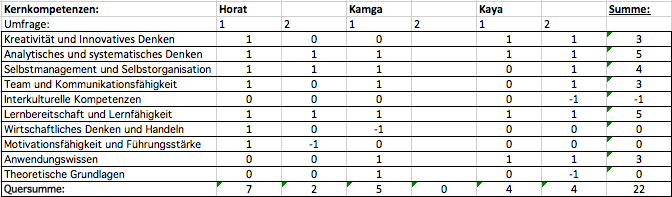
\includegraphics[width=0.7\textwidth]{images/Tabelle_Kernkompetenzen.png}
	\caption{Tabelle Kernkompetenzen}
	\label{fig:tabkernkomp}
\end{figure}

\begin{figure}[ht]
	\centering
	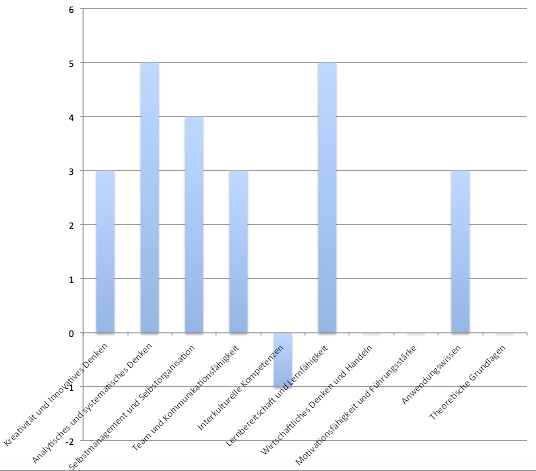
\includegraphics[width=0.7\textwidth]{images/Auswertung_kernkompetenzen.png}
	\caption{Auswertung Kernkompetenzen}
	\label{fig:auswerkomp}
\end{figure}



\subsection{Interview 1}

\subsection{Interview 2}

\subsection{Interview 3}
